\documentclass[CJK,12pt,t]{article}

% Any percent sign marks a comment to the end of the line

% Every latex document starts with a documentclass declaration like this
% The option dvips allows for graphics, 12pt is the font size, and article
%   is the style

%% 使用中文 (CJK package)
\usepackage{CJKutf8}
\usepackage[pdftex]{graphicx}
\usepackage{url}
\usepackage{array}
\usepackage{booktabs}
\usepackage{subfigure}
\usepackage{wrapfig}

\usepackage{amsmath}
\usepackage{amssymb}
\usepackage{amsthm}

% These are additional packages for "pdflatex", graphics, and to include
% hyperlinks inside a document.

\setlength{\oddsidemargin}{0.25in}
\setlength{\textwidth}{6.5in}
\setlength{\topmargin}{0in}
\setlength{\textheight}{8.5in}
\setlength{\parskip}{15pt}
\newcommand{\argmin}[1]{\underset{#1}{\operatorname{arg}\,\operatorname{min}}\;}
\renewcommand{\labelenumi}{\Alph{enumi})}

% These force using more of the margins that is the default style

\begin{document}
\begin{CJK*}{UTF8}{bkai}   %%% ZZZ %%%  <<< 在這裡更改預設中文字型、編碼
% Everything after this becomes content
% Replace the text between curly brackets with your own

%\title{}
%\author{}
%\date{}

% You can leave out "date" and it will be added automatically for today
% You can change the "\today" date to any text you like


%\maketitle

% This command causes the title to be created in the document

\section{主題四: 應用CMFAS架構於輪圈加工應用}
 
		在此主題我們會將CMFAS實際套用於輪圈加工應用,並且敘述CMFAS對於傳統雲端運算的改善。
		
		如果一個企業需要自行組建一個高效能運算叢集,其建置與後續維護的成本必然是一筆不小的數目。從建置時期就必須雇用一個專業人員來進行整體叢集規畫;硬體的成本除了伺服器機台本身,還有機房環境的調控以及機房土地的租賃都是需要被算入的成本,更不用說後期一些硬體設備的汰換、維護與擴建。這種作法最為然所詬病的缺點就是我們無法很彈性地去調整叢集的運算規模,每一次的改變都必須經過繁複的硬體採買與安裝設定程序,大大地減少了調整服務的彈性。

		但是,如果能夠將運算機台交由專業IaaS供應商來維護,像是Windows Azure或是AWS EC2等服務,企業即可以省去上述建置時期的許多麻煩,而且IaaS供應商能夠保證其服務的穩定性,更重要的就是依據IaaS服務的特性,我們只需要去增減向供應商要求的虛擬機台數量,即可非常彈性地去改變我們的運算規模。因此,使得企業可以因應不同的運算情境來調整所需機台數量,在成本與運算效能上取得一個平衡,使資源更有效率地被使用。

		\begin{figure}[ht]
			\begin{center}
				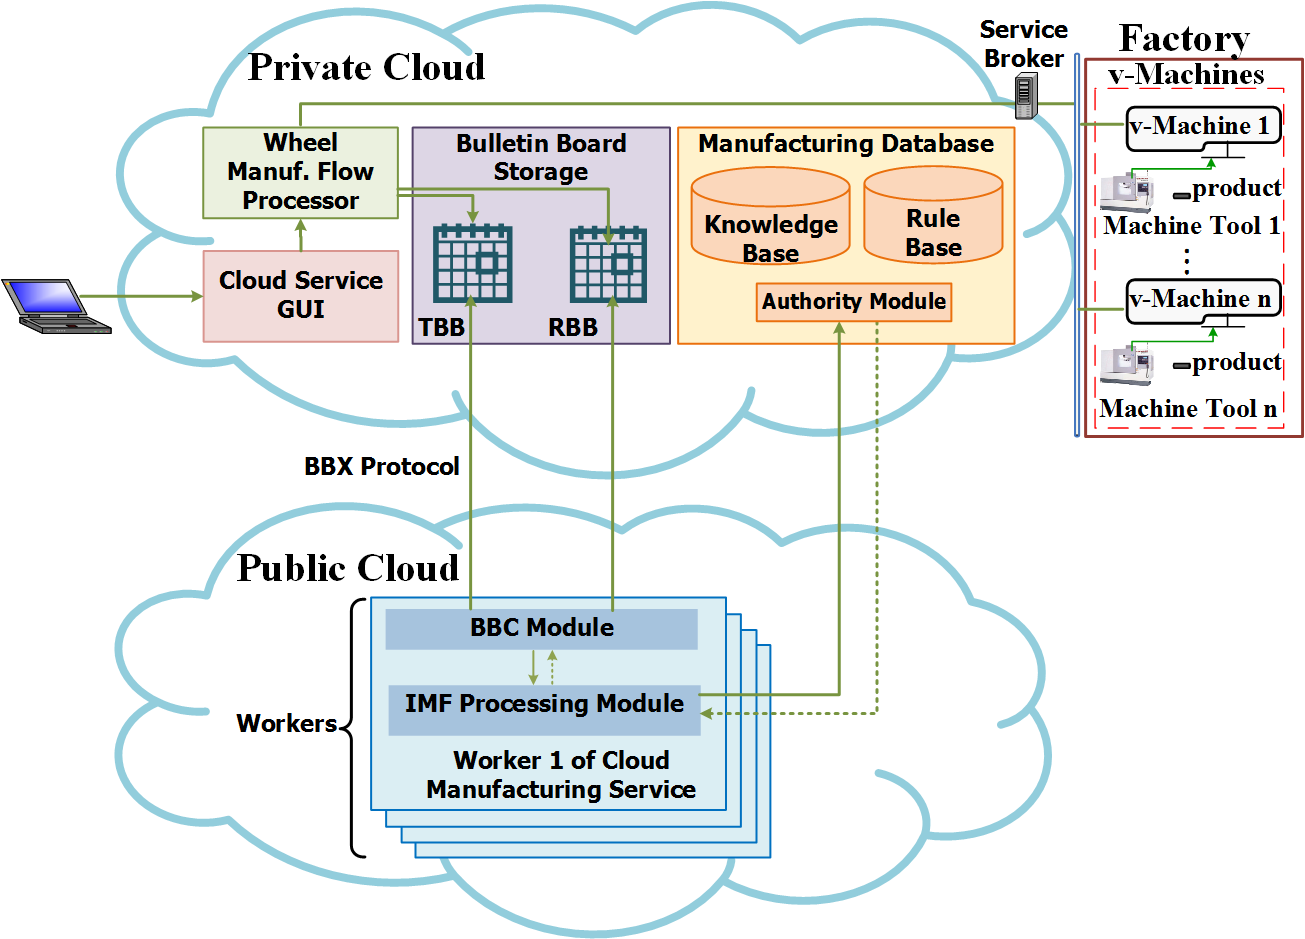
\includegraphics[scale=0.4]{figs/CASE2015.png}
				\caption{CMFAS架構圖}
				\label{cmfas1}
			\end{center}
		\end{figure}

		但對於一般企業而言,必然有著自己的企業機密資料是不放心放在IaaS供應商的機台裡面的。因此,為了能夠於安全地去借用外部之運算資源,我們依照CMFAS原則提出了圖\ref{cmfas1}的架構,針對上述安全性以及規模調整的好處,以下為此架構做更詳盡之說明:
		
		\begin{itemize}
		\setlength{\itemsep}{5pt}
			\item 確保機密資料的安全性:\\
					將具有機密性的資料建立在Manufacturing Database之中。並且建置在我們自行利用VMware所架設的私有雲之中,以此來確保我們對於機密資料的掌握度。\\
					在與IMF Processing Module資料交換之前,透過Authority Module來進行資料加密,來確保在公有雲進行的運算也是安全的。關於資料加密之方法,將於主題六會有更詳盡的解說。

			\item 彈性調製運算規模:\\
				將需要高效能運算的IMF Processing Module建置在可以依照需求調整機台規模的公有雲(例如:Windows Azure或是 AWS EC2等),保持運算資源調配的彈性,方便我們在不同的情境底下,從運算效能與投資成本兩者之間取得一個平衡度。
		\end{itemize}

		我們以輪圈加工業為例,以主題一的CMFAS架構及上述原則來實現一個輪圈加工流程檢測系統。透過檢視NC檔的流程與刀具使用狀況,來預測是否會有碰撞或是刀具使用不當的行為發生,使用本體論之運算來進行刀具使用的修正,使得輪圈加工的流程得以順利進行。

		根據CMFAS框架,我們將本體論所需之知識庫與規則庫建立在Manufacturing Database之中,並將本體論運算與碰撞檢測實作於公有雲之IMF Processing Module中,搭配Cloud Service GUI來蒐集客戶端所送出之加工資訊,以此建構出WD-CAPP(Wheel Design Computer Aided process Planning)系統。

		\vspace{20pt}
		\begin{figure}[ht]
			\begin{center}
				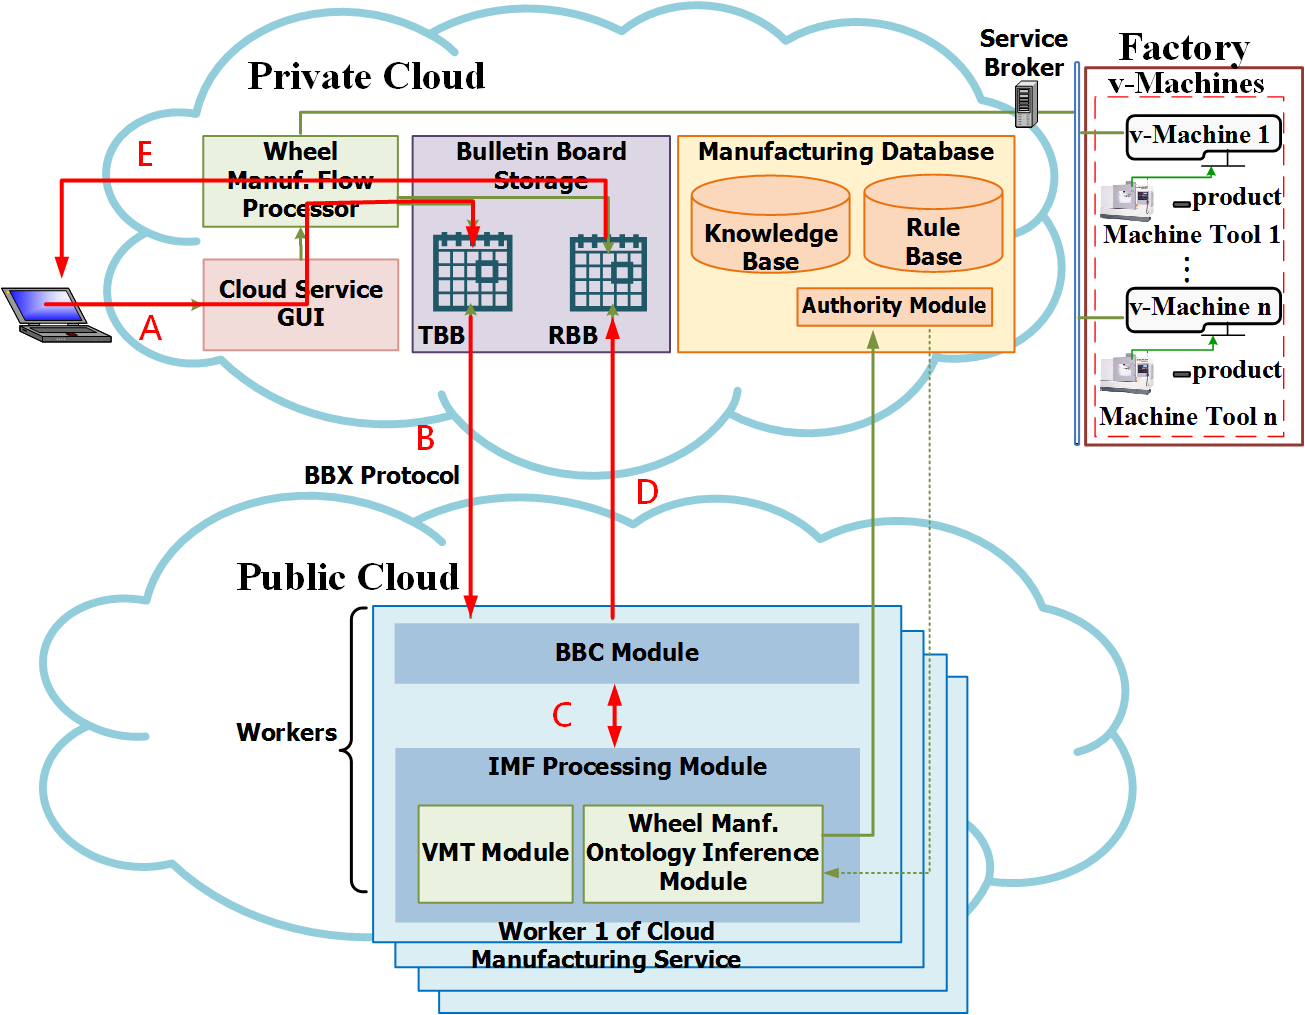
\includegraphics[scale=0.3]{figs/step-wdcaspp.png}
				\caption{WD-CAPP運作流程圖}
				\label{cmfas2}
			\end{center}
		\end{figure}

		圖\ref{cmfas2}為整個WD-CAPP混和雲運作流程,以下為各流程說明

		\begin{enumerate}
		\setlength{\itemsep}{5pt}
			\item 從客戶端將所要使用之NC檔、輪圈加工資訊與欲使用之知識庫等加工資訊發送至Task Bulletin Board(TBB)
			\item 將所有加工資訊自Task Bulletin Board擷取至公有雲之Worker的BBC Module
			\item BBC Module根據加工資訊呼叫需要運作之Manufacturing Function。\\
					透過VMT Module來呼叫碰撞檢測之服務。若遇到刀具將會發生碰撞之情況,BBC Module將會呼叫Wheel Manf. Ontology Interency Module來根據知識庫與規則庫推薦正確的刀具。
			\item BBC Module將檢測結果與刀具推薦列表傳至Result Bulletin Board(RBB)
			\item 客戶端再將檢測結果與刀具推薦列表自Result Bulletin Board擷取下來。
		\end{enumerate}

		根據CMFAS這個框架所建立之加工流程檢測系統擁有極大的彈性調整空間,透過抽換不同的知識庫與規則庫便可以適用於不同地加工情境;調整Authority Module可以讓各個廠房擁有自己獨特的加密方式;最重要的則是根據不同情境的製造規模,來調整Worker數量及運算效能,達到資源最有效率地運用,讓整個加工產線的產能與利潤達到最佳化。
\end{CJK*}
\end{document}